% Options for packages loaded elsewhere
\PassOptionsToPackage{unicode}{hyperref}
\PassOptionsToPackage{hyphens}{url}
%
\documentclass[
]{article}
\usepackage{lmodern}
\usepackage{amssymb,amsmath}
\usepackage{ifxetex,ifluatex}
\ifnum 0\ifxetex 1\fi\ifluatex 1\fi=0 % if pdftex
  \usepackage[T1]{fontenc}
  \usepackage[utf8]{inputenc}
  \usepackage{textcomp} % provide euro and other symbols
\else % if luatex or xetex
  \usepackage{unicode-math}
  \defaultfontfeatures{Scale=MatchLowercase}
  \defaultfontfeatures[\rmfamily]{Ligatures=TeX,Scale=1}
\fi
% Use upquote if available, for straight quotes in verbatim environments
\IfFileExists{upquote.sty}{\usepackage{upquote}}{}
\IfFileExists{microtype.sty}{% use microtype if available
  \usepackage[]{microtype}
  \UseMicrotypeSet[protrusion]{basicmath} % disable protrusion for tt fonts
}{}
\makeatletter
\@ifundefined{KOMAClassName}{% if non-KOMA class
  \IfFileExists{parskip.sty}{%
    \usepackage{parskip}
  }{% else
    \setlength{\parindent}{0pt}
    \setlength{\parskip}{6pt plus 2pt minus 1pt}}
}{% if KOMA class
  \KOMAoptions{parskip=half}}
\makeatother
\usepackage{xcolor}
\IfFileExists{xurl.sty}{\usepackage{xurl}}{} % add URL line breaks if available
\IfFileExists{bookmark.sty}{\usepackage{bookmark}}{\usepackage{hyperref}}
\hypersetup{
  pdftitle={Results of Ordered Likelihood Analysis},
  pdfauthor={Devan Becker},
  hidelinks,
  pdfcreator={LaTeX via pandoc}}
\urlstyle{same} % disable monospaced font for URLs
\usepackage[margin=1in]{geometry}
\usepackage{color}
\usepackage{fancyvrb}
\newcommand{\VerbBar}{|}
\newcommand{\VERB}{\Verb[commandchars=\\\{\}]}
\DefineVerbatimEnvironment{Highlighting}{Verbatim}{commandchars=\\\{\}}
% Add ',fontsize=\small' for more characters per line
\usepackage{framed}
\definecolor{shadecolor}{RGB}{248,248,248}
\newenvironment{Shaded}{\begin{snugshade}}{\end{snugshade}}
\newcommand{\AlertTok}[1]{\textcolor[rgb]{0.94,0.16,0.16}{#1}}
\newcommand{\AnnotationTok}[1]{\textcolor[rgb]{0.56,0.35,0.01}{\textbf{\textit{#1}}}}
\newcommand{\AttributeTok}[1]{\textcolor[rgb]{0.77,0.63,0.00}{#1}}
\newcommand{\BaseNTok}[1]{\textcolor[rgb]{0.00,0.00,0.81}{#1}}
\newcommand{\BuiltInTok}[1]{#1}
\newcommand{\CharTok}[1]{\textcolor[rgb]{0.31,0.60,0.02}{#1}}
\newcommand{\CommentTok}[1]{\textcolor[rgb]{0.56,0.35,0.01}{\textit{#1}}}
\newcommand{\CommentVarTok}[1]{\textcolor[rgb]{0.56,0.35,0.01}{\textbf{\textit{#1}}}}
\newcommand{\ConstantTok}[1]{\textcolor[rgb]{0.00,0.00,0.00}{#1}}
\newcommand{\ControlFlowTok}[1]{\textcolor[rgb]{0.13,0.29,0.53}{\textbf{#1}}}
\newcommand{\DataTypeTok}[1]{\textcolor[rgb]{0.13,0.29,0.53}{#1}}
\newcommand{\DecValTok}[1]{\textcolor[rgb]{0.00,0.00,0.81}{#1}}
\newcommand{\DocumentationTok}[1]{\textcolor[rgb]{0.56,0.35,0.01}{\textbf{\textit{#1}}}}
\newcommand{\ErrorTok}[1]{\textcolor[rgb]{0.64,0.00,0.00}{\textbf{#1}}}
\newcommand{\ExtensionTok}[1]{#1}
\newcommand{\FloatTok}[1]{\textcolor[rgb]{0.00,0.00,0.81}{#1}}
\newcommand{\FunctionTok}[1]{\textcolor[rgb]{0.00,0.00,0.00}{#1}}
\newcommand{\ImportTok}[1]{#1}
\newcommand{\InformationTok}[1]{\textcolor[rgb]{0.56,0.35,0.01}{\textbf{\textit{#1}}}}
\newcommand{\KeywordTok}[1]{\textcolor[rgb]{0.13,0.29,0.53}{\textbf{#1}}}
\newcommand{\NormalTok}[1]{#1}
\newcommand{\OperatorTok}[1]{\textcolor[rgb]{0.81,0.36,0.00}{\textbf{#1}}}
\newcommand{\OtherTok}[1]{\textcolor[rgb]{0.56,0.35,0.01}{#1}}
\newcommand{\PreprocessorTok}[1]{\textcolor[rgb]{0.56,0.35,0.01}{\textit{#1}}}
\newcommand{\RegionMarkerTok}[1]{#1}
\newcommand{\SpecialCharTok}[1]{\textcolor[rgb]{0.00,0.00,0.00}{#1}}
\newcommand{\SpecialStringTok}[1]{\textcolor[rgb]{0.31,0.60,0.02}{#1}}
\newcommand{\StringTok}[1]{\textcolor[rgb]{0.31,0.60,0.02}{#1}}
\newcommand{\VariableTok}[1]{\textcolor[rgb]{0.00,0.00,0.00}{#1}}
\newcommand{\VerbatimStringTok}[1]{\textcolor[rgb]{0.31,0.60,0.02}{#1}}
\newcommand{\WarningTok}[1]{\textcolor[rgb]{0.56,0.35,0.01}{\textbf{\textit{#1}}}}
\usepackage{graphicx}
\makeatletter
\def\maxwidth{\ifdim\Gin@nat@width>\linewidth\linewidth\else\Gin@nat@width\fi}
\def\maxheight{\ifdim\Gin@nat@height>\textheight\textheight\else\Gin@nat@height\fi}
\makeatother
% Scale images if necessary, so that they will not overflow the page
% margins by default, and it is still possible to overwrite the defaults
% using explicit options in \includegraphics[width, height, ...]{}
\setkeys{Gin}{width=\maxwidth,height=\maxheight,keepaspectratio}
% Set default figure placement to htbp
\makeatletter
\def\fps@figure{htbp}
\makeatother
\setlength{\emergencystretch}{3em} % prevent overfull lines
\providecommand{\tightlist}{%
  \setlength{\itemsep}{0pt}\setlength{\parskip}{0pt}}
\setcounter{secnumdepth}{-\maxdimen} % remove section numbering
\usepackage[]{natbib}
\bibliographystyle{plainnat}

\title{Results of Ordered Likelihood Analysis}
\author{Devan Becker}
\date{2021-04-15}

\begin{document}
\maketitle

\begin{Shaded}
\begin{Highlighting}[]
\KeywordTok{library}\NormalTok{(here)}
\end{Highlighting}
\end{Shaded}

\begin{verbatim}
## here() starts at /home/devan/OneDriveUWO/0postdoc/sup
\end{verbatim}

\begin{Shaded}
\begin{Highlighting}[]
\KeywordTok{library}\NormalTok{(dplyr)}
\end{Highlighting}
\end{Shaded}

\begin{verbatim}
## 
## Attaching package: 'dplyr'
\end{verbatim}

\begin{verbatim}
## The following objects are masked from 'package:stats':
## 
##     filter, lag
\end{verbatim}

\begin{verbatim}
## The following objects are masked from 'package:base':
## 
##     intersect, setdiff, setequal, union
\end{verbatim}

\begin{Shaded}
\begin{Highlighting}[]
\KeywordTok{library}\NormalTok{(tidyr)}
\KeywordTok{library}\NormalTok{(stringr)}
\KeywordTok{library}\NormalTok{(ggplot2)}
\NormalTok{ords \textless{}{-}}\StringTok{ }\KeywordTok{lapply}\NormalTok{(}
    \KeywordTok{list.files}\NormalTok{(}\KeywordTok{here}\NormalTok{(}\StringTok{"data/pangordlineages"}\NormalTok{),}
        \DataTypeTok{full.names =} \OtherTok{TRUE}\NormalTok{),}
\NormalTok{    read.csv}
\NormalTok{    ) }\OperatorTok{\%\textgreater{}\%}
\StringTok{    }\KeywordTok{bind\_rows}\NormalTok{() }\OperatorTok{\%\textgreater{}\%}
\StringTok{    }\KeywordTok{separate}\NormalTok{(}\DataTypeTok{col =}\NormalTok{ taxon, }
        \DataTypeTok{into =} \KeywordTok{c}\NormalTok{(}\StringTok{"dummy"}\NormalTok{, }\StringTok{"acc"}\NormalTok{, }\StringTok{"lik"}\NormalTok{, }\StringTok{"subs"}\NormalTok{),}
        \DataTypeTok{sep =} \StringTok{"\_"}\NormalTok{) }\OperatorTok{\%\textgreater{}\%}
\StringTok{    }\KeywordTok{mutate}\NormalTok{(}\DataTypeTok{nsubs =} \KeywordTok{str\_count}\NormalTok{(subs, }\StringTok{"2"}\NormalTok{),}
        \DataTypeTok{lik =} \KeywordTok{as.numeric}\NormalTok{(lik)) }\OperatorTok{\%\textgreater{}\%}
\StringTok{    }\KeywordTok{group\_by}\NormalTok{(acc) }\OperatorTok{\%\textgreater{}\%}
\StringTok{    }\KeywordTok{mutate}\NormalTok{(}\DataTypeTok{order =} \DecValTok{1}\OperatorTok{:}\KeywordTok{n}\NormalTok{()) }\OperatorTok{\%\textgreater{}\%}
\StringTok{    }\KeywordTok{ungroup}\NormalTok{()}
\end{Highlighting}
\end{Shaded}

\begin{Shaded}
\begin{Highlighting}[]
\KeywordTok{ggplot}\NormalTok{(ords) }\OperatorTok{+}
\StringTok{    }\KeywordTok{aes}\NormalTok{(}\DataTypeTok{x =}\NormalTok{ order, }\DataTypeTok{y =}\NormalTok{ lik, }\DataTypeTok{colour =} \KeywordTok{factor}\NormalTok{(acc)) }\OperatorTok{+}\StringTok{ }
\StringTok{    }\KeywordTok{geom\_line}\NormalTok{() }\OperatorTok{+}
\StringTok{    }\KeywordTok{theme}\NormalTok{(}\DataTypeTok{legend.position =} \StringTok{"none"}\NormalTok{)}
\end{Highlighting}
\end{Shaded}

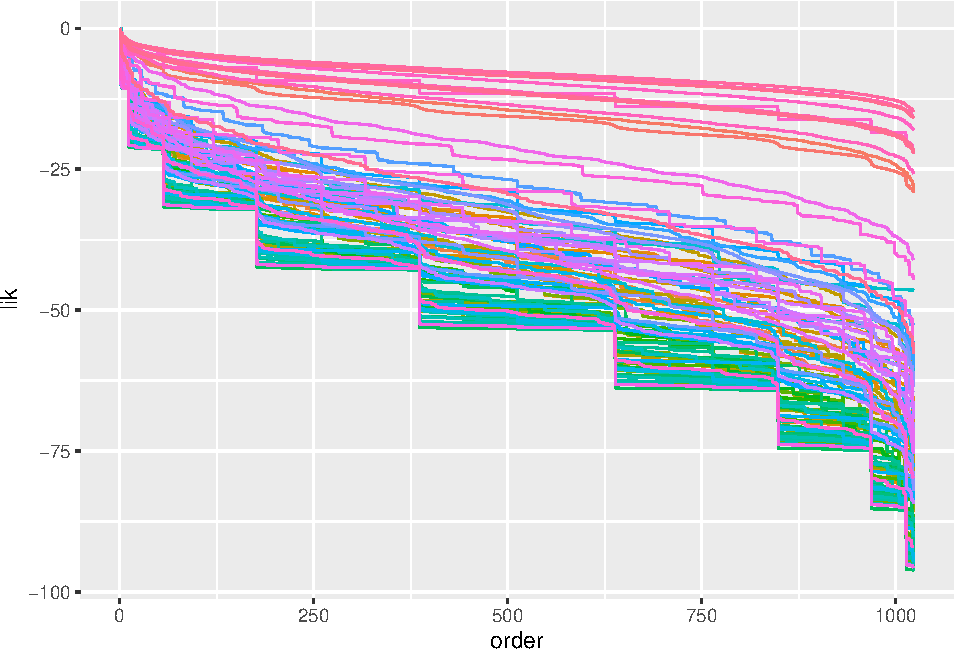
\includegraphics{ord-results_files/figure-latex/change_in_weight-1.pdf}

\begin{Shaded}
\begin{Highlighting}[]
\NormalTok{ords }\OperatorTok{\%\textgreater{}\%}
\StringTok{    }\KeywordTok{group\_by}\NormalTok{(acc, lineage) }\OperatorTok{\%\textgreater{}\%}
\StringTok{    }\KeywordTok{summarise}\NormalTok{(}
        \DataTypeTok{count =} \KeywordTok{n}\NormalTok{(),}
        \DataTypeTok{weight =} \KeywordTok{sum}\NormalTok{(lik),}
        \DataTypeTok{.groups =} \StringTok{"drop"}
\NormalTok{    ) }\OperatorTok{\%\textgreater{}\%}
\StringTok{    }\KeywordTok{group\_by}\NormalTok{(acc) }\OperatorTok{\%\textgreater{}\%}
\StringTok{    }\KeywordTok{summarise}\NormalTok{(}
        \DataTypeTok{unique =} \KeywordTok{length}\NormalTok{(}\KeywordTok{unique}\NormalTok{(lineage)),}
        \DataTypeTok{mode =} \KeywordTok{names}\NormalTok{(}\KeywordTok{sort}\NormalTok{(}\KeywordTok{table}\NormalTok{(lineage)))[}\DecValTok{1}\NormalTok{],}
        \DataTypeTok{mode\_n =} \KeywordTok{max}\NormalTok{(count),}
        \DataTypeTok{mode\_wt =} \KeywordTok{sum}\NormalTok{(weight[lineage }\OperatorTok{==}
\StringTok{            }\KeywordTok{names}\NormalTok{(}\KeywordTok{sort}\NormalTok{(}\KeywordTok{table}\NormalTok{(lineage)))[}\DecValTok{1}\NormalTok{]]),}
        \DataTypeTok{ru =} \KeywordTok{names}\NormalTok{(}\KeywordTok{sort}\NormalTok{(}\KeywordTok{table}\NormalTok{(lineage)))[}\DecValTok{2}\NormalTok{],}
        \DataTypeTok{ru\_wt =} \KeywordTok{sum}\NormalTok{(weight[lineage }\OperatorTok{==}
\StringTok{            }\KeywordTok{names}\NormalTok{(}\KeywordTok{sort}\NormalTok{(}\KeywordTok{table}\NormalTok{(lineage)))[}\DecValTok{2}\NormalTok{]]),}
        \DataTypeTok{.groups =} \StringTok{"drop"}
\NormalTok{    ) }\OperatorTok{\%\textgreater{}\%}
\StringTok{    }\KeywordTok{print}\NormalTok{(}\DataTypeTok{n =} \OtherTok{Inf}\NormalTok{)}
\end{Highlighting}
\end{Shaded}

\begin{verbatim}
## # A tibble: 145 x 7
##     acc         unique mode       mode_n  mode_wt ru    ru_wt
##     <chr>        <int> <chr>       <int>    <dbl> <chr> <dbl>
##   1 ERR4085809       1 B.1          4097  -79030. <NA>     NA
##   2 ERR4204823       1 B.40         4097  -74491. <NA>     NA
##   3 ERR4305816       1 B.3.1        4097 -212360. <NA>     NA
##   4 ERR4307842       1 B.1.1.289    4097 -198114. <NA>     NA
##   5 ERR4363387       1 B.1.222      4097 -217517. <NA>     NA
##   6 ERR4364007       1 B.1.1.29     4097 -204256. <NA>     NA
##   7 ERR4440194       1 B.1          4097 -137463. <NA>     NA
##   8 ERR4440219       1 B.1.1.164    4097 -229343. <NA>     NA
##   9 ERR4440247       1 B.1.1.29     4097 -249809. <NA>     NA
##  10 ERR4440332       1 B.40         4097 -243778. <NA>     NA
##  11 ERR4440354       1 B.1.1.29     4097 -201197. <NA>     NA
##  12 ERR4440373       1 B.40         4097 -199701. <NA>     NA
##  13 ERR4440402       1 B.1.1.29     4097 -250838. <NA>     NA
##  14 ERR4440425       1 B.1.1.29     4097 -124865. <NA>     NA
##  15 ERR4440731       1 B.1          4097 -194927. <NA>     NA
##  16 ERR4664555       1 B.1.1.253    4097 -206957. <NA>     NA
##  17 ERR4667618       1 B.1.1.315    4097 -177257. <NA>     NA
##  18 ERR4692364       1 B.1          4097 -183334. <NA>     NA
##  19 ERR4693034       1 B.1.1.310    4097 -250825. <NA>     NA
##  20 ERR4693061       1 B.23         4097 -208652. <NA>     NA
##  21 ERR4693079       1 B.1.1.310    4097 -219303. <NA>     NA
##  22 ERR4693537       1 B.1.177.7    4097 -176805. <NA>     NA
##  23 ERR4693605       1 B.1.177.3    4097 -232353. <NA>     NA
##  24 ERR4694400       1 B.3          4097 -241241. <NA>     NA
##  25 ERR4694556       1 B.1.1.15     4097 -239395. <NA>     NA
##  26 ERR4694571       1 B.1.1.29     4097 -247301. <NA>     NA
##  27 ERR4694617       1 B.1.1.304    4097 -222814. <NA>     NA
##  28 ERR4759453       1 B.1.1.29     4097 -245753. <NA>     NA
##  29 ERR4869446       1 B.1.160.7    4097 -196927. <NA>     NA
##  30 ERR4869458       1 B.1.177      4097 -193039. <NA>     NA
##  31 ERR4869480       1 B.1.177      4097 -172391. <NA>     NA
##  32 ERR4869487       1 B.1.177      4097 -216110. <NA>     NA
##  33 ERR4869497       1 B.1.1.315    4097 -211230. <NA>     NA
##  34 ERR4890228       1 B.1.1.29     4097 -247440. <NA>     NA
##  35 ERR4890271       1 B.1.1.307    4097 -243703. <NA>     NA
##  36 ERR4890285       1 B.1.523      4097 -247435. <NA>     NA
##  37 ERR4890294       1 B.1.1.29     4097 -250900. <NA>     NA
##  38 ERR4890337       1 B.1.36.17    4097 -251378. <NA>     NA
##  39 ERR4890352       1 B.1.36.17    4097 -258681. <NA>     NA
##  40 ERR4890354       1 B.1          4097 -249937. <NA>     NA
##  41 ERR4890371       1 B.1.36.17    4097 -194502. <NA>     NA
##  42 ERR4890386       1 B.1.177.18   4097 -249264. <NA>     NA
##  43 ERR4890403       1 B.1.177      4097 -244445. <NA>     NA
##  44 ERR4890427       1 B.39         4097 -243567. <NA>     NA
##  45 ERR4891711       1 B.1.36       4097 -250668. <NA>     NA
##  46 ERR4891715       1 B            4097 -247673. <NA>     NA
##  47 ERR4891805       1 B.1.177.6    4097 -239842. <NA>     NA
##  48 ERR4891841       1 B.1          4097 -240721. <NA>     NA
##  49 ERR4891863       1 B.1.1.216    4097 -252343. <NA>     NA
##  50 ERR4891889       1 B.1          4097 -244178. <NA>     NA
##  51 ERR4891898       1 B.1.1.304    4097 -251433. <NA>     NA
##  52 ERR4891916       1 None         4097 -223763. <NA>     NA
##  53 ERR4891988       1 B            4097 -242489. <NA>     NA
##  54 ERR4892048       1 B.1.1.307    4097 -259073. <NA>     NA
##  55 ERR4892066       1 B.1.1.29     4097 -240113. <NA>     NA
##  56 ERR4892112       1 B.39         4097 -246632. <NA>     NA
##  57 ERR4892152       1 B.1.177      4097 -235342. <NA>     NA
##  58 ERR4892200       1 B.1.177.17   4097 -240791. <NA>     NA
##  59 ERR4892203       1 B.1.1.216    4097 -239508. <NA>     NA
##  60 ERR4892293       1 B.1.1.162    4097 -253570. <NA>     NA
##  61 ERR4892339       1 B.1.177      4097 -252963. <NA>     NA
##  62 ERR4892386       1 B.40         4097 -242534. <NA>     NA
##  63 ERR4892392       1 B.1.177      4097 -261658. <NA>     NA
##  64 ERR4892423       1 B.1.523      4097 -232354. <NA>     NA
##  65 ERR4893013       1 B.1          4097 -254046. <NA>     NA
##  66 ERR4893031       1 B.1.177      4097 -251173. <NA>     NA
##  67 ERR4893033       1 B.1.1.307    4097 -255070. <NA>     NA
##  68 ERR4893037       1 B.1.1.29     1025  -50499. <NA>     NA
##  69 ERR4893080       1 B.1.177      4097 -239759. <NA>     NA
##  70 ERR4893138       1 B.1.177.16   4097 -237300. <NA>     NA
##  71 ERR4893184       1 B.1.258      4097 -251877. <NA>     NA
##  72 ERR4893186       1 B.1.1.216    4097 -257503. <NA>     NA
##  73 ERR4893197       1 B.1.177      4097 -252565. <NA>     NA
##  74 ERR4893242       1 B.1.177      4097 -256504. <NA>     NA
##  75 ERR4893353       1 B.1.1.307    4097 -259369. <NA>     NA
##  76 ERR4893393       1 B.1.523      4097 -243247. <NA>     NA
##  77 ERR4999251       1 None         4097 -231451. <NA>     NA
##  78 ERR4999255       1 None         4097 -172688. <NA>     NA
##  79 ERR4999275       1 None         4097 -208182. <NA>     NA
##  80 ERR4999282       1 B            4097 -165933. <NA>     NA
##  81 ERR5060778       1 B.1.177      4097 -209950. <NA>     NA
##  82 ERR5062004       1 B.1.258      4097 -228372. <NA>     NA
##  83 ERR5062062       1 B.1.177      4097 -195607. <NA>     NA
##  84 ERR5062388       1 B.1.1.7      4097 -188059. <NA>     NA
##  85 ERR5062514       1 B.1.1.307    4097 -242281. <NA>     NA
##  86 ERR5062571       1 B.1.177      4097 -254470. <NA>     NA
##  87 ERR5062648       1 B.1.177.4    4097 -210712. <NA>     NA
##  88 ERR5062729       1 B.1.177      4097 -230350. <NA>     NA
##  89 ERR5062935       1 B.1.1.7      4097 -218038. <NA>     NA
##  90 ERR5063143       1 B.1.1.7      4097 -193297. <NA>     NA
##  91 ERR5063165       1 B.1.177.19   4097 -224469. <NA>     NA
##  92 ERR5063539       1 B.1.177      4097 -187660. <NA>     NA
##  93 ERR5063807       1 B.1.1.7      4097 -259703. <NA>     NA
##  94 ERR5063813       1 B.1.177.19   4097 -237048. <NA>     NA
##  95 ERR5063922       1 B.1.177      4097 -217321. <NA>     NA
##  96 ERR5064166       1 B.1.177      4097 -253871. <NA>     NA
##  97 ERR5064294       1 B.1.177      4097 -256003. <NA>     NA
##  98 ERR5064346       1 B.1.1.7      4097 -228953. <NA>     NA
##  99 ERR5064787       1 B.1.177.17   4097 -212447. <NA>     NA
## 100 ERR5064811       1 B.1.1.7      4097 -181307. <NA>     NA
## 101 ERR5069584       1 B.1.1.7      4097 -213096. <NA>     NA
## 102 ERR5069616       1 B.1.1.7      4097 -196001. <NA>     NA
## 103 ERR5069624       1 B.1          1025  -50487. <NA>     NA
## 104 ERR5069871       1 B.1.1.7      4097 -222206. <NA>     NA
## 105 ERR5070060       1 B.1.177      4097 -224395. <NA>     NA
## 106 ERR5070294       1 B.1.1.7      4097 -230383. <NA>     NA
## 107 ERR5074314       1 B.1.160      4097 -153383. <NA>     NA
## 108 ERR5076163       1 B.1.177.19   4097 -190206. <NA>     NA
## 109 ERR5076748       1 B.1.177.19   4097 -162150. <NA>     NA
## 110 ERR5077151       1 B.1.177      4097 -139044. <NA>     NA
## 111 ERR5077411       1 B.1.1.7      4097 -218489. <NA>     NA
## 112 ERR5077618       1 B.1.1.7      4097 -168679. <NA>     NA
## 113 ERR5080893       1 B.1.1.251    4097 -213961. <NA>     NA
## 114 ERR5080897       1 B.1.36.17    4097 -176531. <NA>     NA
## 115 ERR5080913       1 B.1.1.311    4097 -165046. <NA>     NA
## 116 ERR5080918       1 B.1.177      4097 -192261. <NA>     NA
## 117 ERR5081301       1 B.1.177      4097 -212809. <NA>     NA
## 118 ERR5081316       1 B.1.177.15   4097 -181207. <NA>     NA
## 119 ERR5082556       1 B.1.177.7    4097 -224183. <NA>     NA
## 120 ERR5082569       1 B.1.160      4097 -182461. <NA>     NA
## 121 ERR5082576       1 B.1.177      4097 -200961. <NA>     NA
## 122 ERR5082580       1 B.1.177      4097 -184198. <NA>     NA
## 123 ERR5082590       1 B.1.177.4    4097 -180386. <NA>     NA
## 124 ERR5082610       1 B.1.1.7      4097 -197288. <NA>     NA
## 125 ERR5082630       1 B.1.177.7    4097 -196673. <NA>     NA
## 126 ERR5082645       1 B.1.177      4097 -173206. <NA>     NA
## 127 ERR5082664       1 B.1.1.315    4097  -97871. <NA>     NA
## 128 ERR5082674       1 B.1.177.6    4097 -221744. <NA>     NA
## 129 ERR5082695       1 B.1.177      4033 -199157. <NA>     NA
## 130 ERR5082696       1 B.1.1.315    1025  -29492. <NA>     NA
## 131 ERR5082711       1 B.1.177      4097 -109945. <NA>     NA
## 132 ERR5082712       1 B.1.177.7    4097 -211397. <NA>     NA
## 133 SRR12639958      1 None         4097 -249673. <NA>     NA
## 134 SRR12762573      1 A            4097  -56913. <NA>     NA
## 135 SRR13020989      1 B.1.1.273    4097  -49532. <NA>     NA
## 136 SRR13020990      1 A.2.2        4097  -73328. <NA>     NA
## 137 SRR13021027      1 B.1.1.241    4097  -55414. <NA>     NA
## 138 SRR13021032      1 A.2.2        4097  -40781. <NA>     NA
## 139 SRR13021033      1 B.1          4097  -57484. <NA>     NA
## 140 SRR13021035      1 A.2.2        4097  -47671. <NA>     NA
## 141 SRR13021038      1 A.2.2        4097  -56331. <NA>     NA
## 142 SRR13021042      1 A.2.2        4097  -57047. <NA>     NA
## 143 SRR13021047      1 B.1          4097  -60173. <NA>     NA
## 144 SRR13021097      1 A.1          4097  -44760. <NA>     NA
## 145 SRR13092002      1 A.1          4097 -144723. <NA>     NA
\end{verbatim}

\end{document}
